
% ==================================================================
\section{Historical Development of General Circulation Theory}\label{sec:history}
% ==================================================================

% ------------------------------------------------------------------
\subsection{Early Observations: Halley and the Trade Winds}
% ------------------------------------------------------------------

\hisu{무역풍의 발견과 Halley의 관측}

Christopher Columbus's westward voyages (1492--) revealed a remarkably persistent
pattern: steady easterly winds in the low latitudes that reliably carried ships from
Europe toward the Caribbean.  These \textbf{trade winds} became the empirical foundation
of atmospheric science, long before any dynamical theory existed.

\begin{definition}[Trade Winds]
  \tight
  The \emph{trade winds} are the prevailing surface-level easterly winds found in the
  tropics, blowing from the subtropical high-pressure belts toward the equatorial
  low-pressure trough (the Intertropical Convergence Zone, ITCZ).
  \hisu{적도 저압대 쪽으로 부는 지속적인 편동풍; 대항해시대의 핵심 동력}
\end{definition}

\textbf{Edmund Halley} (1656--1742) offered the first physical explanation.
In his 1686 paper, Halley argued that \textgr{differential solar heating} drives the
trade winds: intense heating near the equator causes air to rise, drawing surface air
equatorward from both hemispheres.  He also produced the first known map of surface
winds over the tropical oceans.

\begin{hisublock}
  Halley의 설명은 위도에 따른 solar heating의 차이를 동력으로 제시했다는 점에서 혁명적이었지만,
  왜 바람이 남북이 아닌 동서 방향을 갖는지는 설명하지 못했다 (지구 자전 효과를 고려하지 않음).
\end{hisublock}

\begin{figure}[ht]
  \centering
  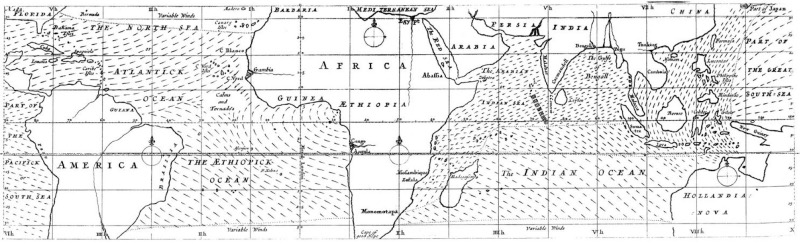
\includegraphics[width=0.85\textwidth]{images/ch01/p03_img01.jpeg}
  \caption{Halley's 1686 map of surface winds over the tropical oceans---the first
    known attempt to chart the global wind pattern from ship observations.
    \hisu{Halley가 1686년에 발표한 열대 해양 표면풍 지도; 관측 기반 최초의 전구 바람 지도}.}
  \label{fig:halley-wind-map}
\end{figure}

% ------------------------------------------------------------------
\subsection{Hadley's Single-Cell Model}
% ------------------------------------------------------------------

\textbf{George Hadley} (1685--1768) addressed the missing piece in his 1735 paper
``Concerning the Cause of the General Trade-Winds.''  His key insight was to incorporate
the \emph{rotation of the Earth}.

\begin{definition}[Thermally Direct Cell]\label{def:thermally-direct}
  \tight
  A \emph{thermally direct cell} is a meridional overturning circulation in which
  warm air rises in the region of greatest heating and cold air sinks in the region
  of greatest cooling.  The sense of overturning is ``consistent with'' the thermal
  forcing.
  \hisu{열적으로 직접적인 순환: 따뜻한 곳에서 상승, 차가운 곳에서 하강}
\end{definition}

Hadley's reasoning proceeded as follows:
\begin{enumerate}
  \item Strong solar heating at the equator causes air to rise.
  \item At upper levels, this air flows poleward.
  \item Conservation of angular momentum requires that this poleward-moving air
    acquire a westerly (west-to-east) component, since it originated at a larger
    distance from the rotation axis.
  \item The return flow at the surface, moving equatorward, is deflected
    \emph{westward}, producing the observed easterly trade winds.
\end{enumerate}

\subsubsection{Angular Momentum Argument}

The absolute angular momentum per unit mass of a parcel on a rotating sphere is
\begin{equation}\label{eq:ang-mom}
  M = (u + \Omega a \cos\phi)\,a\cos\phi,
\end{equation}
where $u$ is the zonal wind, $\Omega$ the planetary rotation rate, $a$ the Earth's
radius, and $\phi$ the latitude.  If a parcel at rest at the equator ($\phi = 0$,
$u = 0$) moves to latitude $\phi$ while conserving $M$, then
\begin{equation}\label{eq:ang-mom-conserve}
  u(\phi) = \Omega a \frac{\sin^2\phi}{\cos\phi}.
\end{equation}

\begin{hisublock}
  Hadley는 적도에서 극까지 하나의 거대한 thermally direct cell을 상상했지만,
  실제 Hadley circulation은 열대(위도 $\sim$30$^\circ$)에 국한된다.
  이유: 각운동량 보존에 의해 상층 서풍이 너무 강해져서 중위도에서는
  baroclinic instability에 의해 순환이 깨진다 (Sec.~\ref{subsec:rotation} 참조). \\
  Ref: (Lorenz, 1983, \textit{Bull.\ Amer.\ Meteor.\ Soc.})
\end{hisublock}

\begin{figure}[ht]
  \centering
  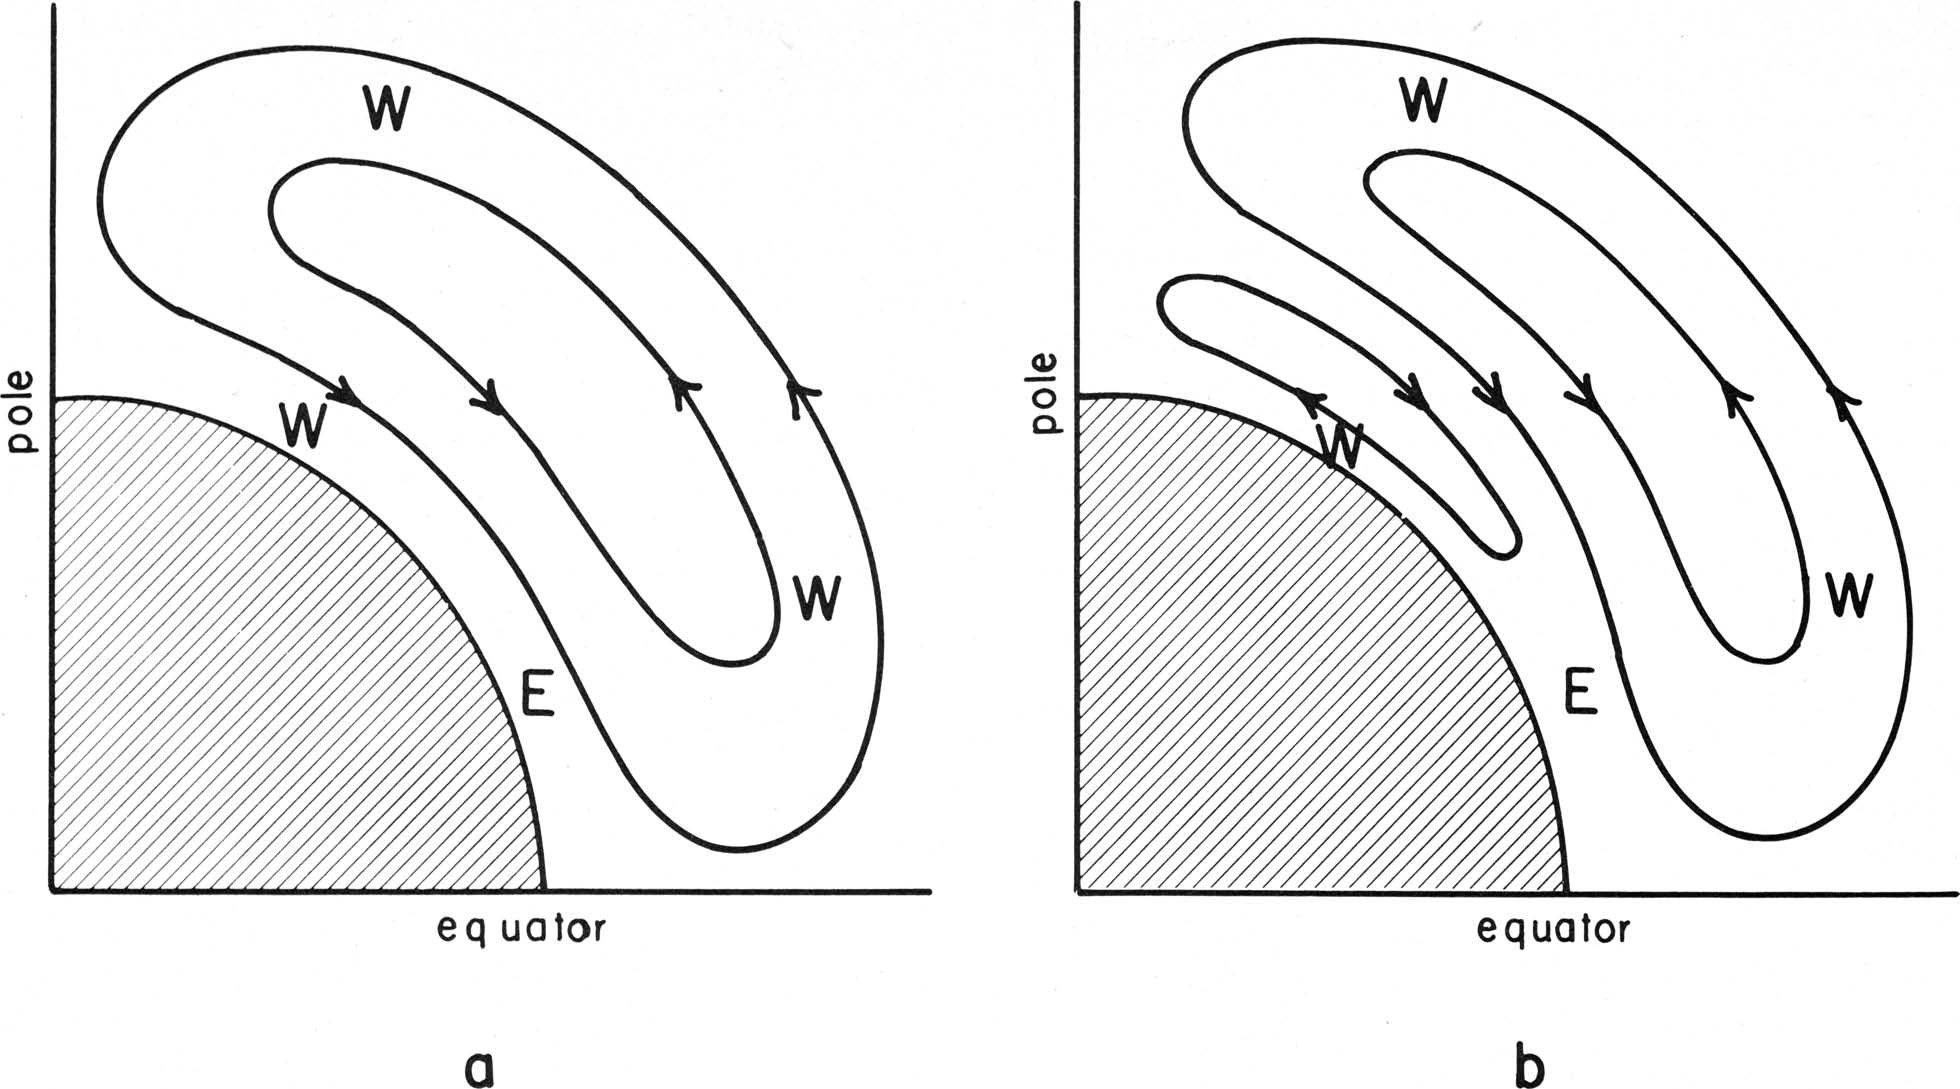
\includegraphics[width=0.85\textwidth]{images/ch01/p08_img01.jpeg}
  \caption{Schematic of Hadley's single thermally direct cell: warm air rises at the
    equator, flows poleward aloft, sinks at the pole, and returns equatorward at the
    surface. \hisu{Hadley의 단일 직접순환 모식도: 적도 상승 $\to$ 상층 극향 $\to$ 극 하강 $\to$ 지표 적도향}.}
  \label{fig:hadley-single-cell}
\end{figure}

% ------------------------------------------------------------------
\subsection{Thomson and Ferrel: The Three-Cell Model}
% ------------------------------------------------------------------

The single-cell picture survived for over a century before being challenged.

\textbf{James Thomson} (1857) recognized that what we now call the \textgr{Coriolis
force}---the apparent deflection experienced by air moving over a rotating
Earth---would prevent a simple equator-to-pole overturning.  He proposed a
\emph{multi-cell} structure.

\textbf{William Ferrel} (1856, 1859) independently developed a \textbf{three-cell
model} of the meridional circulation:

\begin{multicols}{2}
\begin{itemize}
  \item \textbf{Hadley cell} (0--30$^\circ$): thermally direct
  \item \textbf{Ferrel cell} (30--60$^\circ$): thermally \emph{indirect}
  \item \textbf{Polar cell} (60--90$^\circ$): thermally direct
\end{itemize}
\columnbreak
\begin{hisublock}
  Hadley cell $\to$ 직접순환 \\
  Ferrel cell $\to$ 간접순환 \\
  Polar cell $\to$ 직접순환 \\
  3개 cell이 맞물려서 전구 순환 형성
\end{hisublock}
\end{multicols}

\begin{definition}[Thermally Indirect Cell]\label{def:thermally-indirect}
  \tight
  A \emph{thermally indirect cell} is a meridional overturning circulation whose
  sense of overturning is \emph{opposite} to that which thermal forcing alone would
  produce: relatively cool air rises on the poleward side, while relatively warm
  air sinks on the equatorward side.  The Ferrel cell is the canonical example.
  \hisu{열적 강제와 반대 방향으로 순환하는 cell; 중위도 Ferrel cell이 대표적}
\end{definition}

\begin{hisublock}
  Thomson은 multi-cell 구조를 제안했으나 thermally indirect cell의 개념을 명확히 구분하지 못했다.
  Ferrel은 Thomson과 달리 thermally indirect cell (Ferrel cell)을 극지방까지 확장하지 않았으며,
  중위도에 국한된 간접순환으로 올바르게 인식했다.
\end{hisublock}

\begin{figure}[ht]
  \centering
  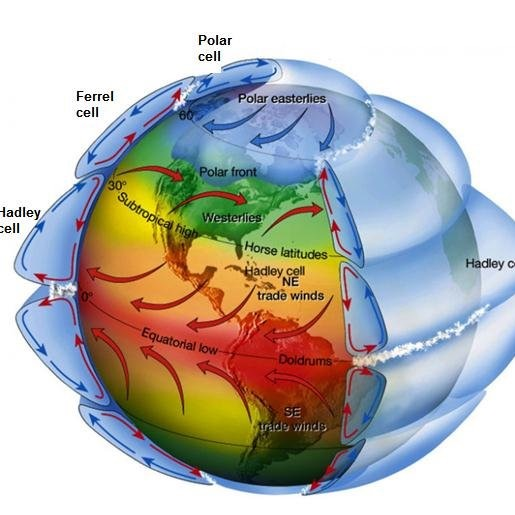
\includegraphics[width=0.85\textwidth]{images/ch01/p12_img01.jpeg}
  \caption{The three-cell model of the meridional circulation: Hadley cell
    (thermally direct, 0--30$^\circ$), Ferrel cell (thermally indirect, 30--60$^\circ$),
    and Polar cell (thermally direct, 60--90$^\circ$), shown on a 3-D globe view.
    \hisu{3-cell 모델의 3차원 모식도: Hadley, Ferrel, Polar cell의 배치와 지표풍 방향을 확인하라}.}
  \label{fig:three-cell-model}
\end{figure}

\begin{remark}
  The Ferrel cell is not driven by direct thermal forcing.  Rather, it is maintained
  by the convergence of eddy momentum fluxes associated with mid-latitude baroclinic
  waves.  In this sense, it is a fundamentally \emph{eddy-driven} circulation.
\end{remark}

\newpage
% ==================================================================
\section{The Nature of the Problem}\label{sec:nature}
% ==================================================================

% ------------------------------------------------------------------
\subsection{Differential Heating}\label{subsec:diff-heating}
% ------------------------------------------------------------------

The starting point of any theory of the general circulation is the observation that
the Earth's climate system is in approximate \textbf{radiative equilibrium} at the
top of the atmosphere (TOA):
\begin{equation}\label{eq:global-balance}
  \overline{Q_{\mathrm{abs}}} = \overline{F_{\mathrm{OLR}}},
\end{equation}
where the overbar denotes a global and annual mean.  The absorbed solar radiation
$Q_{\mathrm{abs}}$ must, on average, equal the outgoing longwave (infrared) radiation
$F_{\mathrm{OLR}}$.

\begin{hisublock}
  전지구 평균적으로 흡수되는 태양 에너지 = 방출되는 적외선 에너지.
  하지만 \textit{위도별로} 보면 이 균형이 깨진다 --- 그것이 순환의 근본 원인.
\end{hisublock}

The crucial feature is the \textgr{latitude dependence}:
\begin{itemize}
  \item \textbf{Absorbed solar radiation} $Q_{\mathrm{abs}}(\phi)$ is \emph{strongly}
    latitude-dependent, peaking near the equator.
    \hisu{입사 태양에너지: 위도에 강하게 의존 (적도 $\gg$ 극)}
  \item \textbf{Outgoing longwave radiation} $F_{\mathrm{OLR}}(\phi)$ is only
    \emph{weakly} latitude-dependent, because the meridional temperature gradient
    is much smaller than it would be in radiative equilibrium.
    \hisu{방출 적외선: 위도 의존성이 약함 (대기-해양 순환이 열을 수송하기 때문)}
\end{itemize}

\noindent This produces a systematic \textbf{radiation surplus} at low latitudes and a
\textbf{radiation deficit} at high latitudes:
\begin{equation}\label{eq:net-rad}
  R_{\mathrm{net}}(\phi) = Q_{\mathrm{abs}}(\phi) - F_{\mathrm{OLR}}(\phi)
  \begin{cases}
    > 0 & \text{(tropics: surplus)}, \\
    < 0 & \text{(high latitudes: deficit)}.
  \end{cases}
\end{equation}

\subsubsection{Daily-Mean TOA Insolation}

The daily-mean insolation at the top of the atmosphere depends on latitude $\phi$ and
the solar declination angle $\delta_s$:
\begin{equation}\label{eq:insolation}
  \bar{S}(\phi) = \frac{S_0}{\pi}
  \bigl( h_0 \sin\phi\,\sin\delta_s + \cos\phi\,\cos\delta_s\,\sin h_0 \bigr),
\end{equation}
where $S_0$ is the solar constant and $h_0$ is the hour angle at sunset.

\begin{figure}[ht]
  \centering
  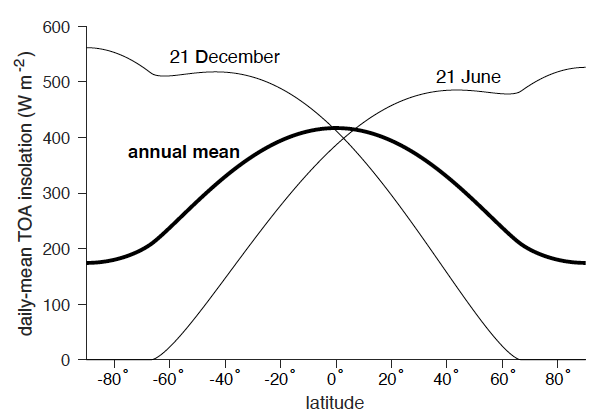
\includegraphics[width=0.85\textwidth]{images/ch01/p17_img01.png}
  \caption{Daily-mean top-of-atmosphere insolation as a function of latitude for June
    solstice, December solstice, and the annual mean. Note the polar maximum during
    the respective summer solstice due to 24-hour daylight.
    \hisu{하지(June)에는 북극에서 일사량 최대, 동지(Dec)에는 남극에서 최대; 연평균은 적도 최대}.}
  \label{fig:toa-insolation}
\end{figure}

\begin{hisublock}
  June solstice: 일사량이 북극에서 최대 (24시간 일조 효과).
  December solstice: 남극에서 최대.
  Annual mean: 적도 부근에서 최대, 극에서 최소.
  결론적으로 위도에 따른 net radiation의 불균형이 대기-해양 순환의 원동력.
\end{hisublock}

% ------------------------------------------------------------------
\subsection{The Atmosphere as a Heat Engine}\label{subsec:heat-engine}
% ------------------------------------------------------------------

The general circulation can be viewed as a \textbf{thermodynamic heat engine} that
converts thermal energy into kinetic energy.

\begin{definition}[Atmospheric Heat Engine]
  \tight
  The atmosphere absorbs heat $Q_A$ at a relatively \emph{warm} temperature
  $T_{\mathrm{warm}}$ (primarily in the tropics, dominated by latent heat release)
  and rejects heat $Q_L$ at a relatively \emph{cool} temperature
  $T_{\mathrm{cool}}$ (primarily in the extratropics, through radiative cooling).
  The net mechanical work done per cycle is
  \begin{equation}\label{eq:work-output}
    W = Q_A - Q_L.
  \end{equation}
  \hisu{열대에서 열 흡수 $\to$ 중고위도에서 열 방출 $\to$ 그 차이가 역학적 일(운동에너지)로 전환}
\end{definition}

On a thermodynamic $T$--$s$ (temperature--entropy) diagram, the atmospheric cycle
traces a clockwise loop.  The area enclosed by this loop equals the net work output
$W$.

\begin{figure}[ht]
  \centering
  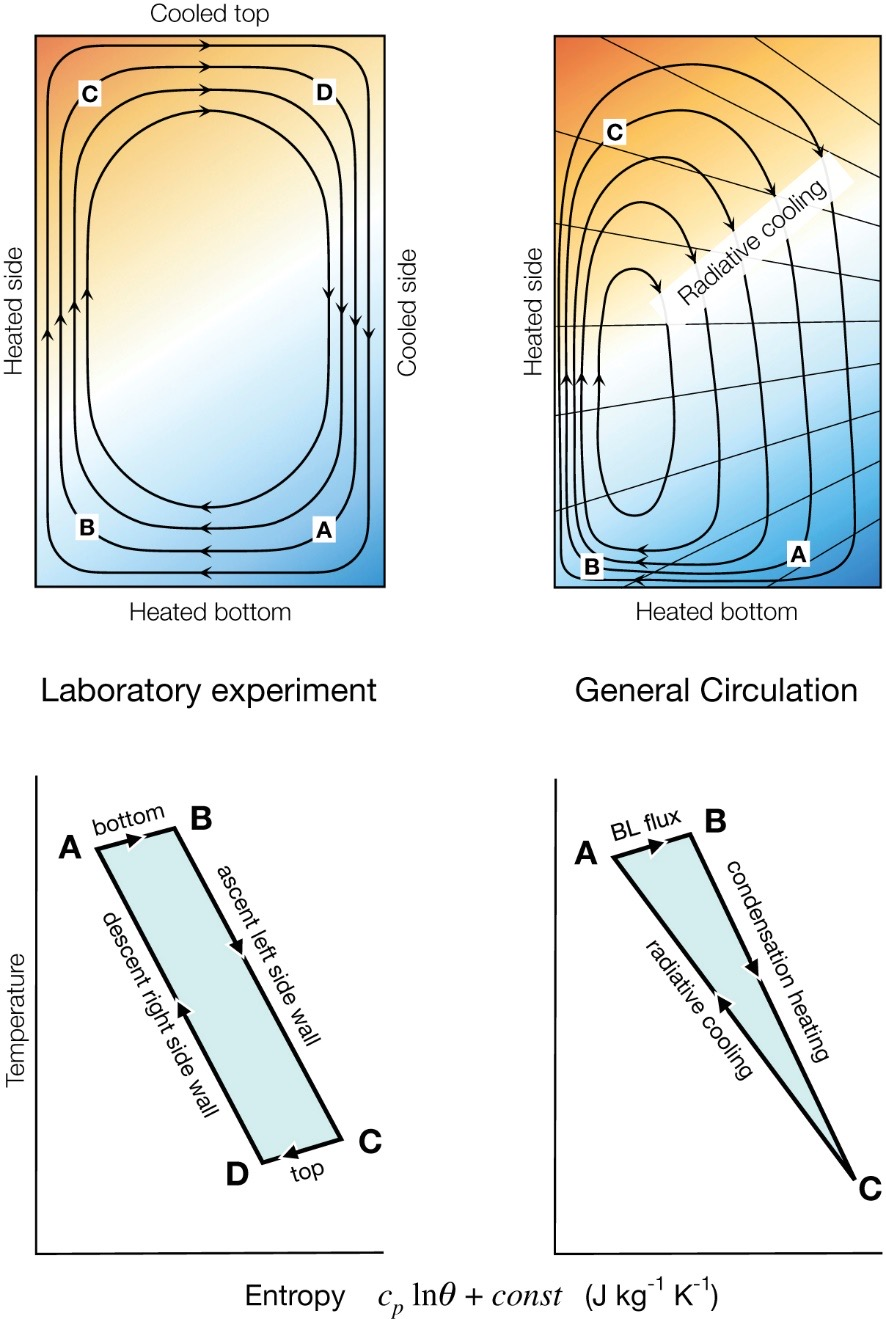
\includegraphics[width=0.85\textwidth]{images/ch01/p46_img01.jpeg}
  \caption{$T$--$s$ diagram of the general circulation: the clockwise loop encloses an
    area equal to the net work $W$ produced by the atmospheric heat engine, shown
    alongside the analogous laboratory experiment.
    \hisu{대기 열기관의 $T$--$s$ 다이어그램; 시계방향 루프의 면적 = 순 역학적 일 $W$}.}
  \label{fig:ts-diagram}
\end{figure}

The specific entropy $s$ of dry air is related to potential temperature $\theta$ by
\begin{equation}\label{eq:entropy-theta}
  s = c_p \ln\theta + \text{const},
\end{equation}
where $c_p$ is the specific heat at constant pressure.

\begin{remark}
  The efficiency of the atmospheric heat engine is far below the Carnot limit.
  Typical estimates give an efficiency of only a few percent, reflecting the fact that
  most of the absorbed energy is re-radiated rather than converted to kinetic energy.
  \hisu{대기의 열효율은 Carnot 효율보다 훨씬 낮다 --- 대부분의 에너지는 다시 복사로 방출됨}
\end{remark}

% ------------------------------------------------------------------
\subsection{Available Potential Energy}\label{subsec:ape}
% ------------------------------------------------------------------

Not all potential energy in the atmosphere is available for conversion to kinetic
energy.  This motivates the concept of \textbf{available potential energy} (APE).

\begin{definition}[Available Potential Energy (APE)]\label{def:ape}
  \tight
  The \emph{available potential energy} (Lorenz, 1955) is the difference between the
  total potential energy of the atmosphere and the minimum potential energy that could
  be achieved by an adiabatic rearrangement of mass to a statically stable reference
  state:
  \begin{equation}\label{eq:ape}
    \mathrm{APE} = \mathrm{PE}_{\mathrm{actual}} - \mathrm{PE}_{\mathrm{ref}}.
  \end{equation}
  Only this fraction is available for conversion to kinetic energy.
  \hisu{전체 위치에너지 중 운동에너지로 전환 가능한 부분만이 APE; 실제로는 매우 작은 비율 ($\sim$0.5\%)}
\end{definition}

The energy conversion chain in the atmosphere proceeds as follows:
\begin{equation}\label{eq:energy-chain}
  \underbrace{\mathrm{APE}}_{\text{differential heating}}
  \;\xrightarrow{\text{baroclinic processes}}\;
  \underbrace{\mathrm{KE}}_{\text{winds}}
  \;\xrightarrow{\text{friction}}\;
  \underbrace{\text{Internal Energy}}_{\text{heat}}.
\end{equation}

\begin{hisublock}
  정상 상태(steady state)에서:
  $$\text{APE} \to \text{KE 전환율} = \text{마찰에 의한 KE 소멸율}.$$
  대기 운동에너지의 거의 전부는 수평 규모 $\gtrsim 100$\,km의 수평풍에 존재한다.
  연직 운동의 KE 기여는 무시할 수 있을 정도로 작다.
\end{hisublock}

\begin{remark}
  The atmosphere maintains a quasi-steady kinetic energy budget: the rate of
  generation of KE from APE is balanced by the rate of frictional dissipation.
  Observationally, virtually all KE resides in the horizontal wind on scales larger
  than $\sim$100\,km.
\end{remark}

\newpage
% ==================================================================
\section{Heuristic Models}\label{sec:heuristic}
% ==================================================================

% ------------------------------------------------------------------
\subsection{Radiative--Convective Equilibrium}\label{subsec:rce}
% ------------------------------------------------------------------

Before considering the full three-dimensional circulation, it is useful to consider
two idealised one-dimensional equilibria.

\begin{definition}[Pure Radiative Equilibrium]\label{def:rad-eq}
  \tight
  A state in which the net emission of infrared radiation at every level equals
  the absorbed solar radiation at that level:
  \begin{equation}
    \frac{\partial F_{\mathrm{net}}}{\partial z} = Q_{\mathrm{solar}}(z)
    \quad \text{at each altitude } z.
  \end{equation}
  \hisu{각 고도에서 적외선 방출 = 흡수된 태양복사. 대류 없이 복사만으로 결정되는 온도 프로파일.}
\end{definition}

The pure radiative equilibrium temperature profile yields an unrealistically high
surface temperature ($\sim$330\,K) and an extremely steep lapse rate in the lower
troposphere --- far exceeding the threshold for convective instability.

\begin{definition}[Radiative--Convective Equilibrium (RCE)]\label{def:rce}
  \tight
  A state in which the vertical temperature profile is determined jointly by
  \emph{radiative transfer} and \emph{convective adjustment}.  Where the radiative
  equilibrium lapse rate exceeds a critical value (typically the moist or dry
  adiabatic lapse rate), convection acts to restore the lapse rate to the critical
  value.
  \hisu{복사 평형의 비현실적 온도 기울기를 대류가 조정 $\to$ radiative-convective equilibrium}
\end{definition}

\begin{figure}[ht]
  \centering
  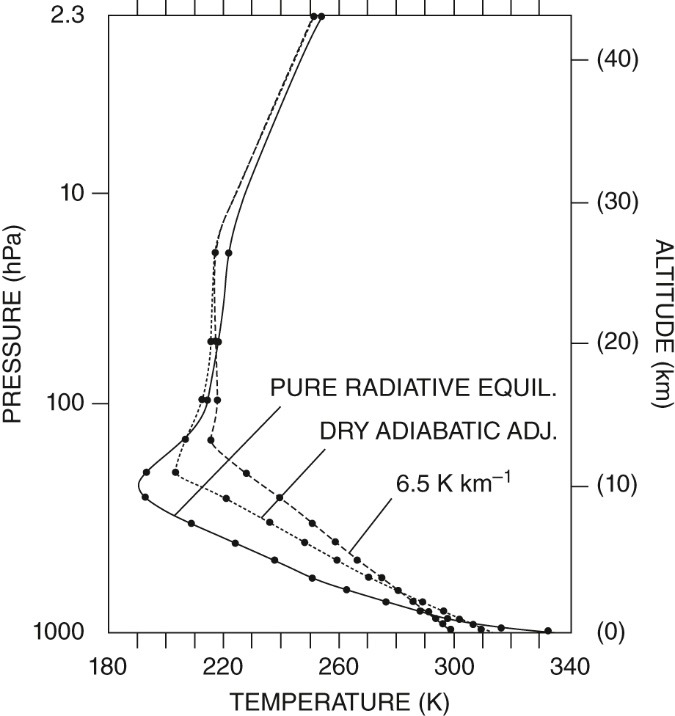
\includegraphics[width=0.85\textwidth]{images/ch01/p27_img01.jpeg}
  \caption{Vertical temperature profiles from Manabe \& Strickler (1964): pure
    radiative equilibrium (dashed) versus radiative--convective equilibrium (solid).
    The radiative-only profile produces an unrealistically steep lapse rate near the
    surface; convective adjustment restores a more realistic profile.
    \hisu{순수 복사 평형(dashed)은 지표 근처 기온감률이 비현실적으로 급함; 대류 조정 후(solid) 현실적 프로파일로 변함}.}
  \label{fig:rce-profiles}
\end{figure}

\begin{hisublock}
  순수 복사 평형(pure radiative equilibrium)은 지표면 온도가 비현실적으로 높고,
  하부 대류권의 기온 감률이 대류 불안정 임계값을 크게 초과한다.
  대류 조정(convective adjustment)이 필요하며, 이것이 RCE의 핵심 아이디어이다.\\
  Ref: (Manabe and Strickler, 1964)
\end{hisublock}

% ------------------------------------------------------------------
\subsection{The Cycling of Mechanical Energy}\label{subsec:cycling}
% ------------------------------------------------------------------

A useful thought experiment illustrates how differential heating generates
mechanical energy.

\subsubsection{Two-Fluid Thought Experiment}

Consider a container divided by a vertical partition into two halves, each filled
with an \emph{immiscible fluid} of different density ($\rho_1 > \rho_2$).

\begin{enumerate}
  \item \textbf{Initial state.}  Dense fluid on the left, light fluid on the right.
    The centre of mass is at some height $z_{\mathrm{cm}}$.
  \item \textbf{Partition removed.}  The dense fluid slides under the light fluid.
    An overturning circulation develops.
  \item \textbf{Final state.}  Dense fluid on the bottom, light fluid on top.
    The centre of mass has dropped: $\Delta z_{\mathrm{cm}} < 0$.
\end{enumerate}

The potential energy released equals the kinetic energy generated (which is then
dissipated by friction):
\begin{equation}\label{eq:two-fluid}
  \Delta \mathrm{PE} = -\int \rho\, g\, \Delta z_{\mathrm{cm}} \, dV
  \;\longrightarrow\; \mathrm{KE} \;\longrightarrow\; \text{Internal Energy (friction)}.
\end{equation}

\begin{hisublock}
  이것이 바로 Hadley circulation의 아날로그:
  적도에서 아래쪽이 가열되고 (가벼운 유체 생성), 극에서 상부가 냉각됨 (무거운 유체 생성).
  $\to$ 밀도차에 의한 overturning $\to$ PE가 KE로 전환.
\end{hisublock}

\begin{figure}[ht]
  \centering
  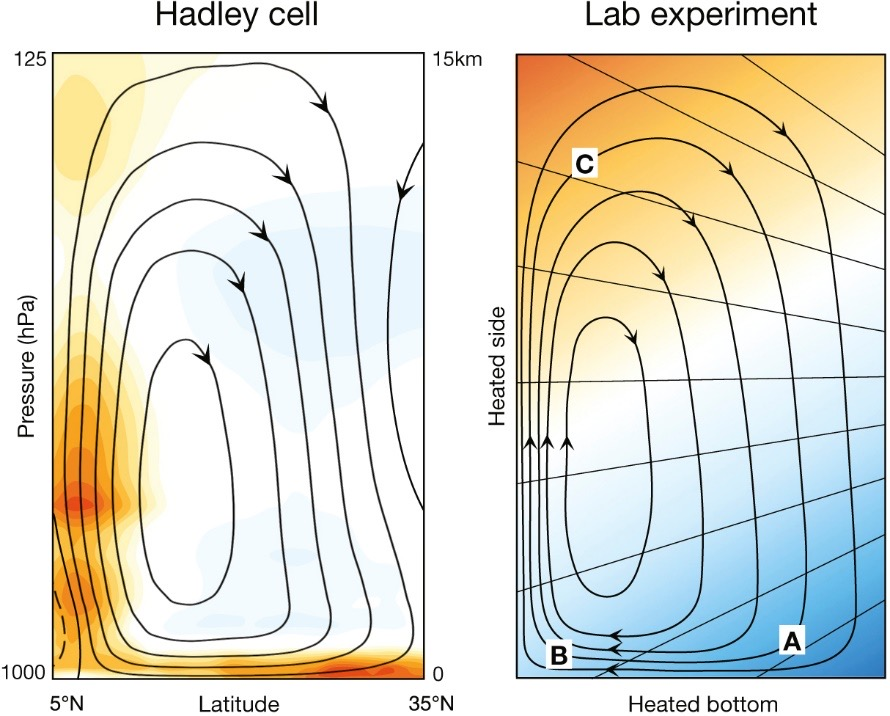
\includegraphics[width=0.85\textwidth]{images/ch01/p35_img01.jpeg}
  \caption{Laboratory experiment: steady-state thermally driven overturning circulation
    in a non-rotating annulus heated from below on one side and cooled from above on
    the other.
    \hisu{비회전 실험 수조에서의 열적 직접순환; 한쪽 가열 + 반대쪽 냉각 $\to$ 정상상태 overturning 발생}.}
  \label{fig:lab-thermal-circulation}
\end{figure}

\subsubsection{Maintenance Requirements}

In the absence of continued forcing, the overturning would cease once the
stratification reaches a stable equilibrium (dense below, light above).
\textgr{Sustained circulation requires both horizontal and vertical gradients of
diabatic heating}:
\begin{itemize}
  \item \textbf{Horizontal gradient:} equator-to-pole differential heating
    creates the meridional density (temperature) gradient.
  \item \textbf{Vertical gradient:} heating at low levels and cooling at upper levels
    continuously destabilises the stratification, maintaining the overturning.
\end{itemize}

\hisu{수평 경도 $+$ 연직 경도 둘 다 있어야 순환이 유지된다. 하나만으로는 정상 상태 순환 불가능.}

% ------------------------------------------------------------------
\subsection{The Influence of Planetary Rotation}\label{subsec:rotation}
% ------------------------------------------------------------------

\subsubsection{Timescales and the Dominance of Rotation}

The radiative relaxation timescale of the troposphere is
\begin{equation}\label{eq:tau-rad}
  \tau_{\mathrm{rad}} \sim 30 \;\text{days},
\end{equation}
which is much longer than the rotation period ($\sim$1 day).  This means that the
Coriolis force has ample time to influence the developing circulation, and the
tidal (diurnal) response is secondary.

\begin{hisublock}
  복사 이완 시간($\sim$30일) $\gg$ 자전 주기($\sim$1일)
  $\to$ Coriolis force가 대기 순환의 구조를 근본적으로 결정한다.
  (만약 자전이 없다면 단순한 적도--극 순환이 될 것)
\end{hisublock}

\subsubsection{Spin-Up Thought Experiment on an Aquaplanet}

The influence of rotation can be understood through a conceptual spin-up experiment
(Held, 2019, Ch.~6, \textit{Meteorological Monographs}):

\begin{enumerate}
  \item[\textbf{(a)}] \textbf{Non-rotating planet.}
    Differential heating drives a simple, hemispheric-scale, equator-to-pole
    thermally direct overturning (one Hadley cell per hemisphere spanning the
    entire latitude range).
    \hisu{자전 없음 $\to$ 단순한 적도-극 직접 순환 (Hadley의 원래 구상)}

  \item[\textbf{(b)}] \textbf{Introduce rotation $\to$ pressure redistribution.}
    As flow develops, the Coriolis force deflects poleward upper-level flow to the
    east and equatorward surface flow to the west.  Pressure gradients are
    redistributed by the evolving wind field.
    \hisu{자전 도입 $\to$ Coriolis 편향 $\to$ 기압장 재배치}

  \item[\textbf{(c)}] \textbf{Geostrophic adjustment $\to$ zonal flow.}
    The flow adjusts toward \emph{geostrophic balance}: the Coriolis force balances
    the pressure gradient force.  The circulation becomes predominantly
    \emph{zonal} (east--west), governed by the \textbf{thermal wind relation}:
    \begin{equation}\label{eq:thermal-wind}
      f \frac{\partial u_g}{\partial z}
      = -\frac{g}{T_0}\frac{\partial T}{\partial y},
    \end{equation}
    where $f = 2\Omega\sin\phi$ is the Coriolis parameter, $u_g$ the geostrophic
    zonal wind, and $\partial T/\partial y$ the meridional temperature gradient.
    \hisu{열풍(thermal wind): 남북 온도 경도가 있으면 상층으로 갈수록 서풍 증가}

  \item[\textbf{(d)}] \textbf{Baroclinic instability.}
    As the meridional temperature gradient steepens under continued differential
    heating, the jet stream intensifies until it reaches a critical shear.
    At that point the zonally symmetric state becomes unstable to wave-like
    perturbations.
\end{enumerate}

\begin{figure}[ht]
  \centering
  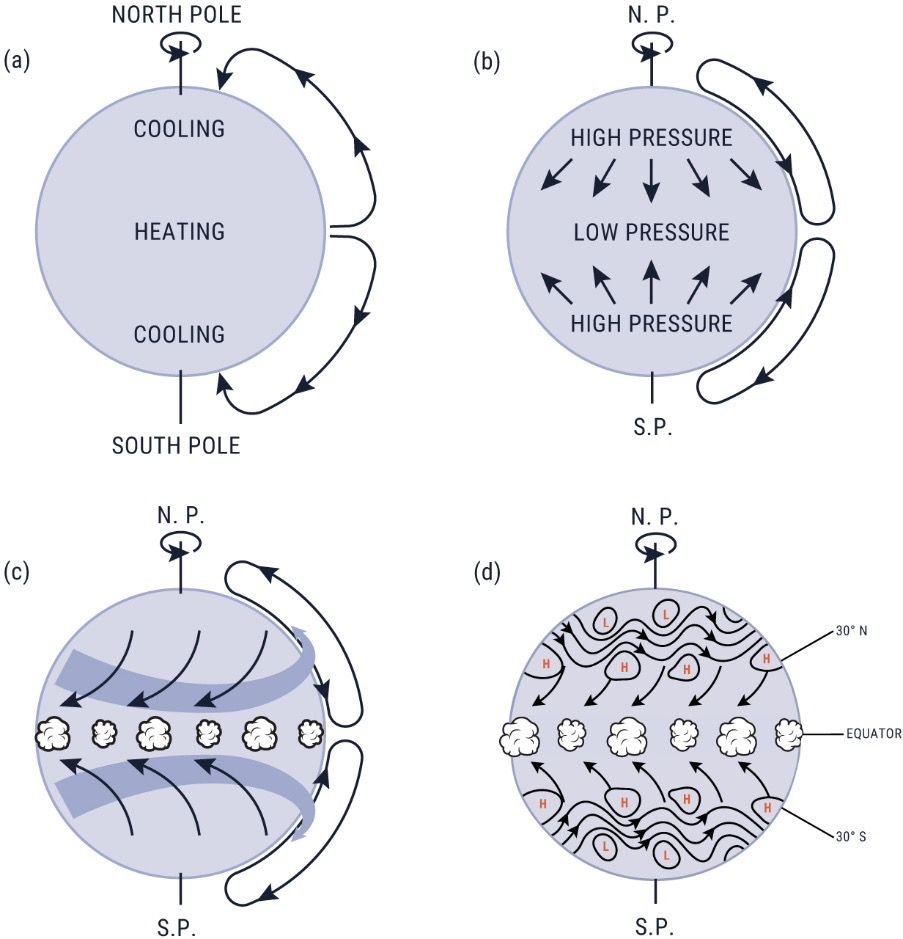
\includegraphics[width=0.85\textwidth]{images/ch01/p51_img01.jpeg}
  \caption{Four-panel spin-up experiment on an aquaplanet: (a) non-rotating thermally
    direct cell, (b) introduction of Coriolis deflection, (c) geostrophic adjustment
    producing strong zonal flow, (d) onset of baroclinic instability breaking the
    zonal symmetry.
    \hisu{(a) 비회전 직접순환 $\to$ (b) Coriolis 편향 $\to$ (c) 지균 조정 $\to$ (d) 경압 불안정 발생; 순환 구조가 단계적으로 복잡해짐}.}
  \label{fig:spin-up-experiment}
\end{figure}

\begin{definition}[Baroclinic Instability]\label{def:baroclinic}
  \tight
  \emph{Baroclinic instability} is the hydrodynamic instability that arises when
  the vertical shear of the zonal wind (equivalently, the meridional temperature
  gradient via thermal wind balance) exceeds a critical threshold.
  It is the primary mechanism by which the zonally symmetric Hadley circulation
  breaks down in the extratropics.
  \begin{itemize}
    \item Fastest-growing mode: synoptic-scale waves with wavelength
      $\sim$3500--4000\,km.
    \item These waves (mid-latitude cyclones and anticyclones) accomplish most of the
      poleward heat and momentum transport in the extratropics.
  \end{itemize}
  \hisu{경압 불안정: Hadley cell의 한계를 넘어선 위도에서 대칭적 순환이 파동으로 깨짐.
  가장 빨리 성장하는 파장 $\sim$3500\,km $\to$ 중위도 저기압/고기압의 규모와 일치}
\end{definition}

\begin{hisublock}
  정리하면, 전구 대기 순환의 핵심 문제는 다음과 같다:
  \begin{enumerate}
    \item 위도별 복사 불균형이 적도--극 온도 경도를 만든다.
    \item 대기는 열기관으로서 이 온도 경도를 이용해 운동에너지를 생성한다.
    \item 지구 자전으로 인해 단순한 직접 순환은 열대에 국한되고 (Hadley cell),
          중위도에서는 경압 불안정이 지배한다.
    \item 최종 결과: three-cell structure + synoptic-scale wave activity.
  \end{enumerate}
  Ref: (Held, 2019, Ch.~6, \textit{Meteorological Monographs})
\end{hisublock}
